\vspace{-5mm}
\section{Introduction}
% Introduce test-time reasoning and self-consistency

Recent progress in large language model (LLM) reasoning has shown that performance on complex tasks can be improved not only by scaling model parameters, but also by allocating more computation at test time. In this paper, \textit{test time} refers to the inference stage of LLMs, where model parameters are fixed and computation is allocated to solve each input. Test-time reasoning methods, such as Chain-of-Thought (CoT) prompting~\cite{wei2022chain}, verifier-guided reasoning~\cite{cobbe2021training}, iterative refinement~\cite{madaan2024self, paul2024refiner}, and search-based decoding~\cite{xie2024self}, improve model outputs by eliciting intermediate reasoning steps or applying additional procedures before producing the final answer. Recent studies on test-time scaling and efficient reasoning highlight a growing concern that additional test-time computation can lead to verbose, repetitive, or low-utility reasoning tokens, making token economy and latency critical bottlenecks for practical deployment~\cite{zhang2025testtimescaling, wang2025efficientreasoning, sui2025stopoverthinking}. Therefore, improving LLM reasoning is not only a matter of scaling test-time compute, but also of using this compute more efficiently.

% Token redundancy and latency of self-consistency

\begin{figure*}[h]
\vspace{-5mm}
\centering
\begin{minipage}[t]{0.45\textwidth}
    \setlength{\abovecaptionskip}{+2mm}
    \centering
    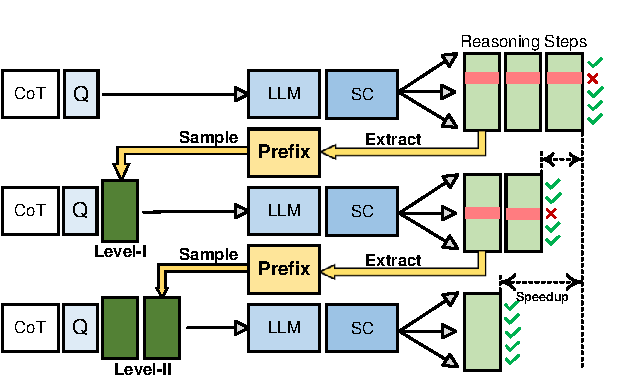
\includegraphics[width=\linewidth]{figures/path-consistency.pdf}
    \caption{Path-consistency extracts high-confidence reasoning prefixes from early sampled paths and reuses them to guide subsequent branches, reducing redundant test-time token generation.}
    \label{fig:path-consistency-simple}
\end{minipage}
\hspace{+2mm}
\begin{minipage}[t]{0.45\textwidth}
\setlength{\abovecaptionskip}{+2mm}
    \centering
    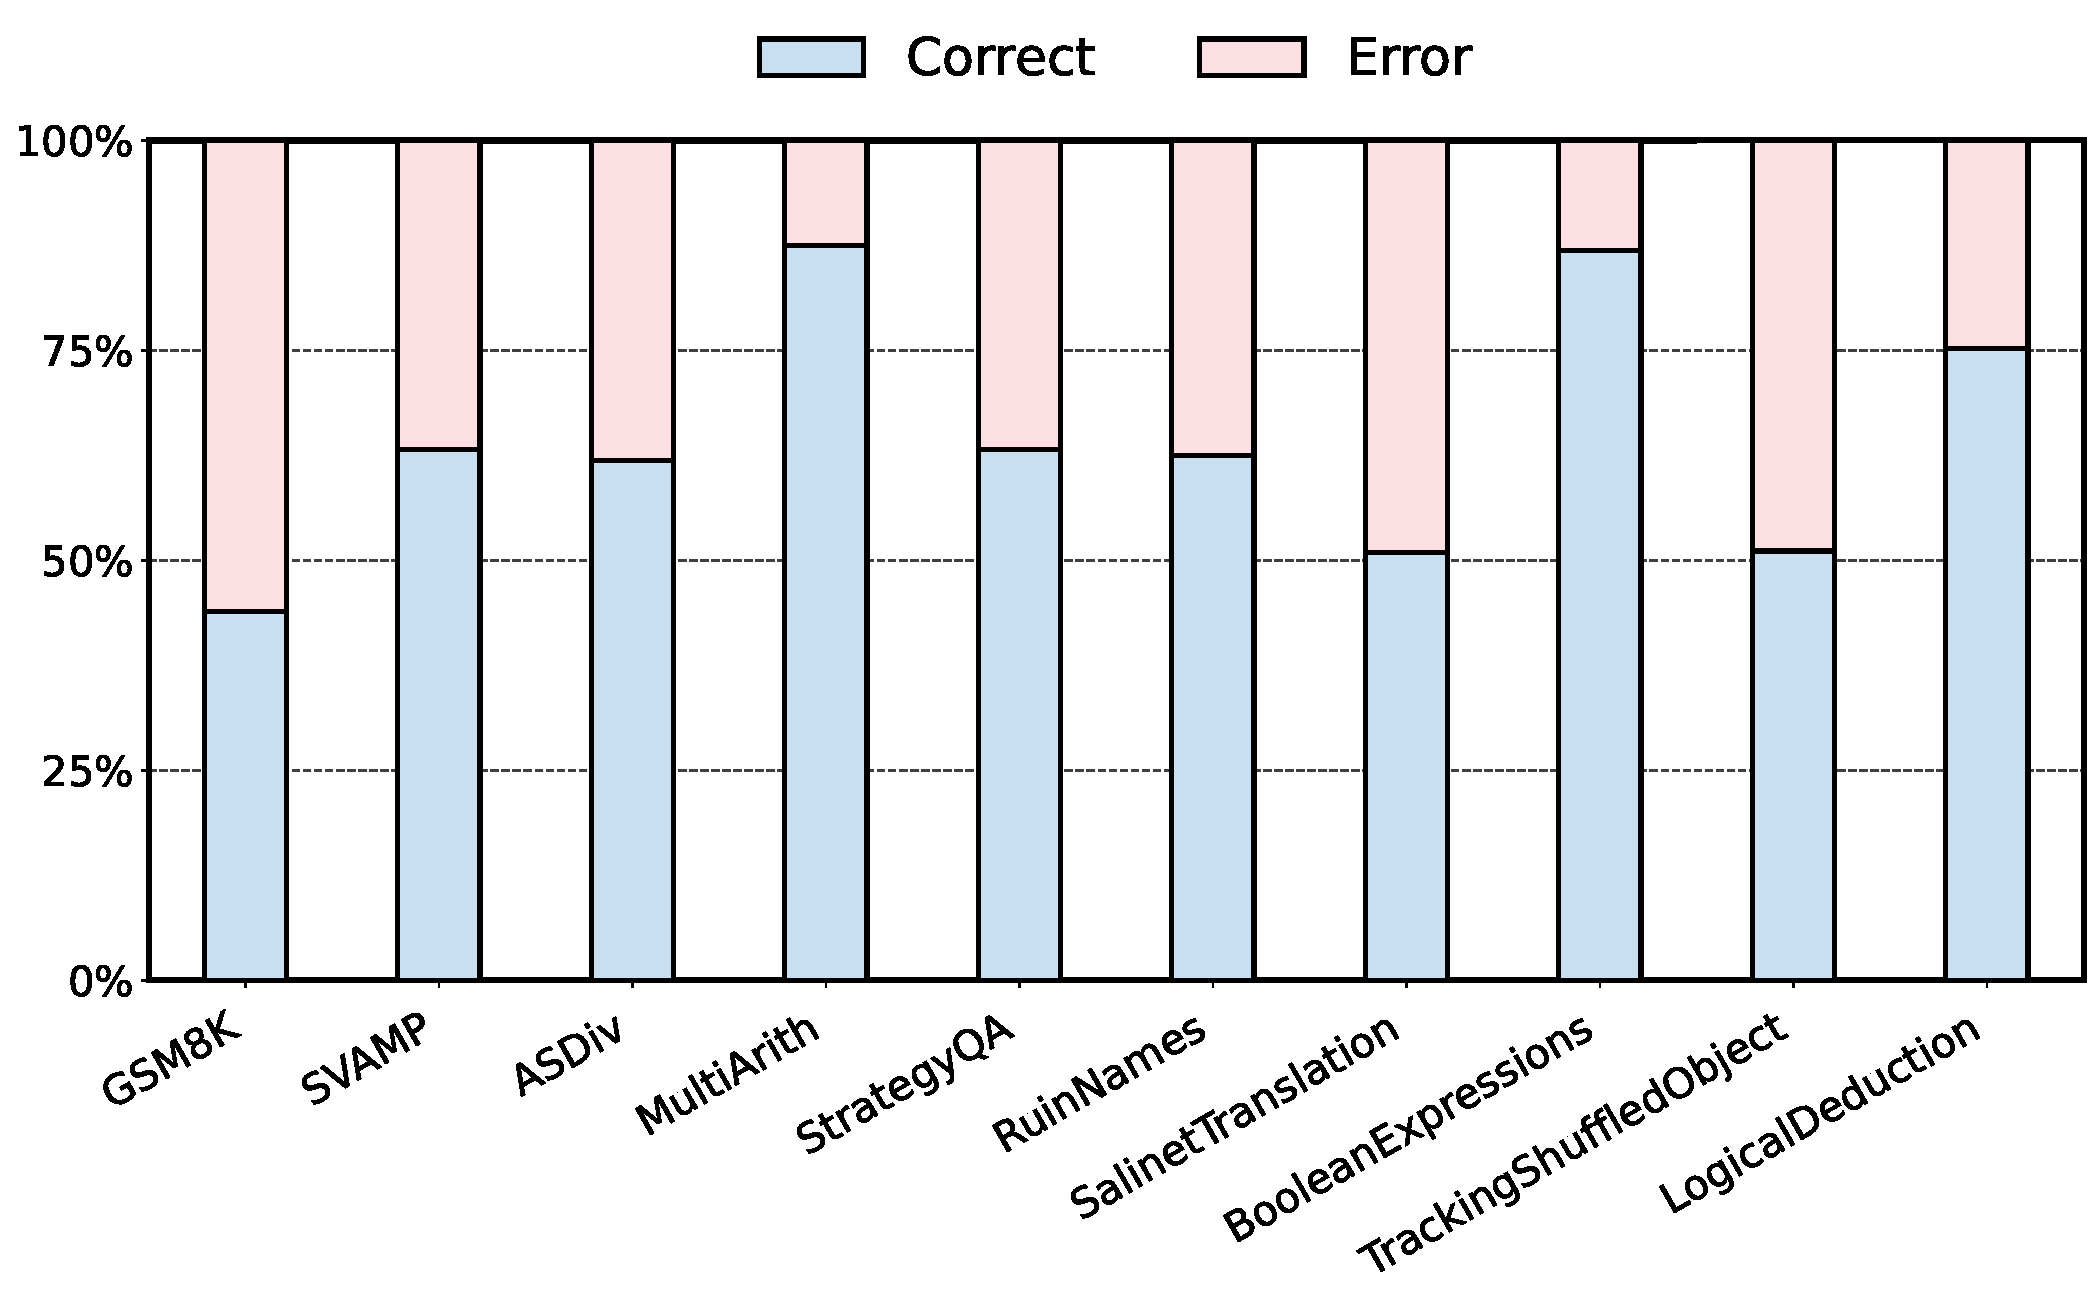
\includegraphics[width=\linewidth]{figures/Characterization.pdf}
    \caption{Token allocation in standard self-consistency. A substantial fraction of test-time tokens is spent on paths that eventually produce incorrect answers.}
    \label{fig:characterization}
\end{minipage}
\vspace{-5mm}
\end{figure*}

Self-consistency~\cite{wang2022self} is a representative test-time reasoning strategy for improving the reliability of CoT-based reasoning. Instead of relying on a single greedy trajectory, it samples multiple reasoning paths for a given input and aggregates their final answers through majority voting. Although this strategy improves the reliability of test-time reasoning, it scales compute in a relatively naive way because each sampled branch is generated as an independent full reasoning path. As the number of branches increases, token consumption and latency grow almost linearly. Moreover, many generated tokens may contribute little to the final answer, because some branches lead to incorrect answers while others repeat similar intermediate reasoning. As shown in \cref{fig:characterization}, a considerable portion of tokens in standard self-consistency is spent on paths that eventually produce incorrect answers. This observation motivates a central question of whether we can preserve the diversity benefit of multi-path sampling while reducing the marginal token cost of later branches.

To address this inefficiency, we propose \textit{path-consistency}, a prefix-guided self-consistency method for token-efficient test-time reasoning. As illustrated in \cref{fig:path-consistency-simple}, path-consistency extracts high-confidence partial reasoning paths from early samples and reuses them as prefixes to condition subsequent generations. Instead of generating every branch from scratch, later samples can start from a promoted prefix and only generate the remaining reasoning steps. In this way, path-consistency reduces redundant token generation while retaining the multi-path sampling structure of self-consistency.

Path-consistency has three practical advantages. First, it improves token efficiency by reducing the number of newly generated tokens in later branches, rather than simply terminating the sampling process early. Second, it requires no model training, fine-tuning, or architecture modification, and the only additional operations are lightweight confidence evaluation and prefix extraction. Third, it is model-agnostic and can be applied to different autoregressive LLMs as a test-time component. These properties make path-consistency complementary to existing sampling-based reasoning methods.

We evaluate path-consistency on ten benchmarks covering arithmetic reasoning~\cite{cobbe2021training, patel2021nlp, miao2020diverse, roy2015solving}, commonsense reasoning~\cite{geva2021did}, and symbolic reasoning~\cite{suzgun-etal-2023-challenging}. Across these tasks, path-consistency reduces inference latency by an average of 28.7\% on arithmetic reasoning, 20.9\% on commonsense reasoning, and 20.3\% on symbolic reasoning, while largely preserving the accuracy of standard self-consistency. These results suggest that reusing intermediate reasoning prefixes is a practical way to improve the efficiency of test-time compute, providing an alternative to naively increasing the number of independently generated reasoning paths.